\documentclass[journal]{IEEEtran}
\usepackage{amsmath}
\usepackage{amssymb}
\usepackage{booktabs}
\usepackage{graphicx}
\usepackage{url}
\usepackage[hidelinks]{hyperref}
\hypersetup{
  pdftitle={Falsification-Guided Layer Repair for Deep Graph Neural Networks},
  pdfauthor={Anonymous Authors},
  pdfsubject={Real-data pilot and falsification protocol for deep graph neural networks}
}

\title{Falsification-Guided Layer Repair for Deep Graph Neural Networks}

\author{Anonymous Authors}

\begin{document}

\maketitle

\begin{abstract}
We evaluate, rather than assume, a falsification-guided layer-repair hypothesis for deep graph neural networks. Energy, effective rank, and local gradient transmission are treated as correlated candidate observables that select a repair mask, and causal location validity is tested against matched controls. The supplied implementation trained 27 real conditions on the public Planetoid Cora split over three seeds using one NVIDIA RTX A6000. Plain accuracy fell from $0.6660 \pm 0.0079$ at depth 2 to $0.2087 \pm 0.0255$ at depth 8. At depth 16, targeted PairNorm reached $0.5913 \pm 0.0595$, uniform PairNorm reached $0.5887 \pm 0.0592$, and wrong-location PairNorm reached $0.6373 \pm 0.0580$. Targeted minus uniform was $0.0027$ with a descriptive 95\% $t$ interval of $[-0.0467,0.0520]$; targeted minus wrong location was $-0.0460$ with interval $[-0.2979,0.2059]$. The target and wrong masks had Jaccard overlap 0.875, and three seeds are underpowered for confirmatory inference. The pilot demonstrates depth degradation and repair viability in this deliberately failing model, but it does not validate layer localization, repair-type prescription, or efficiency. The contribution is a transparent falsification protocol and a negative real-data pilot rather than a journal-scale effectiveness result.
\end{abstract}

\begin{IEEEkeywords}
deep graph neural networks, falsification, gradient transmission, oversmoothing, representation rank, reproducibility
\end{IEEEkeywords}

\section{Introduction}

\IEEEPARstart{G}{raph} convolutional networks aggregate information through repeated neighborhood mixing \cite{kipf2017gcn}. Increasing depth enlarges the nominal receptive field, but deep message-passing networks often become difficult to optimize or lose discriminative structure. Oversmoothing has been the dominant explanation, yet contemporary work warns that mitigating smoothing is not sufficient for expressivity \cite{rusch2023survey}, disputes whether aggregation is the main culprit \cite{park2025fallacy}, proposes rank as a different lens on representation collapse \cite{zhang2026rank}, and derives connections among gradient attenuation, smoothing, and oversquashing \cite{arroyo2025bridging}. These developments make a multi-observable diagnosis scientifically useful as a hypothesis, but not defensible as a novelty claim by itself.

This study asks a narrower, falsifiable question: can measurements taken at individual layers predict where a known repair should be applied? A diagnostic can correlate with failure without locating the layers whose modification causes recovery. The pilot holds treatment cardinality fixed while swapping one treated and one untreated layer. Because the target contains 15 of 16 layers, each wrong-location mask shares 14 treated layers with the target: intersection 14, union 16, Jaccard overlap 0.875, and symmetric difference 2. The manipulation is therefore too weak to identify location and must be replaced by low-overlap controls in a confirmatory study.

The pilot was executed on a single NVIDIA RTX A6000 using the public Planetoid Cora split \cite{yang2016planetoid}. The main result is negative. The fixed selector chose PairNorm from layer 2 onward in each depth-16 seed. That condition recovered much of the untreated performance loss, but a same-cardinality wrong-location control obtained a higher mean. Three seeds cannot establish general success or failure; they show only that the present evidence does not validate the diagnosed location.

The contributions are as follows. First, the study replaces a universal collapse-depth rule with a directionally valid local gradient-transmission statistic. Second, it separates repair viability, location validity, and repair-type prescription. Third, it defines matched controls and quantifies why the present wrong-location manipulation is insufficiently separated. Fourth, it reports the negative A6000 pilot without converting it into a positive localization claim. Fifth, it specifies a confirmatory design with low-overlap masks, equal tuning budgets, held-out test evaluation, complete epoch logging, and explicit claim-retirement rules.

\begin{table}[t]
\caption{Claim audit for the present pilot.}
\label{tab:claim-audit}
\centering
\footnotesize
\setlength{\tabcolsep}{2pt}
\begin{tabular}{p{0.24\columnwidth}p{0.45\columnwidth}p{0.20\columnwidth}}
\toprule
Claim & Pilot evidence & Status \\
\midrule
Depth degradation & Observed on Cora with a plain GCN & Descriptive \\
Repair viability & Repaired runs exceed paired plain runs & Pilot only \\
Layer localization & Targeted does not beat wrong location & Unsupported \\
Repair prescription & Unequal tuning and a wide interval & Unsupported \\
Efficiency & No epoch count or synchronized timing & Not testable \\
\bottomrule
\end{tabular}
\end{table}

\section{Related Work and Novelty Boundary}

\subsection{Smoothing, Rank, and Gradient Flow}

PairNorm preserves pairwise variation without adding trainable parameters \cite{zhao2019pairnorm}, while GCNII combines initial residuals and identity mappings to train deep GCNs \cite{chen2020gcnii}. DeepGCNs transfer residual and dense connections to graph networks and explicitly motivate them by vanishing gradients \cite{li2019deepgcns}. These methods already connect architectural intervention to depth degradation.

The proposed observables cannot be presented as three orthogonal causes. Zhang \emph{et al.} argue that numerical or effective rank can reveal oversmoothing when energy-based metrics do not \cite{zhang2026rank}. Arroyo \emph{et al.} provide a unified view of vanishing gradients, smoothing, and oversquashing \cite{arroyo2025bridging}. Park \emph{et al.} argue that smoothing has sometimes been confused with ordinary trainability \cite{park2025fallacy}. We therefore treat energy, rank, and gradient transmission as correlated candidate observables whose causal specificity must be tested.

\subsection{Adaptive Depth}

Jumping Knowledge networks combine representations from different neighborhood ranges on a per-node basis \cite{xu2018jk}. GAMLP learns node-adaptive combinations of multiple propagation depths \cite{zhang2022gamlp}. Adaptive Message Passing learns depth and message filtering in a variational framework \cite{errica2025amp}. Per-node depth is therefore not a new idea. A diagnostic may instead contribute an externally auditable selection rule, but that contribution depends on a successful localization test.

\subsection{Benchmark Rigor}

Platonov \emph{et al.} show that duplicate nodes in Chameleon and Squirrel can cause leakage and propose a modern heterophily suite \cite{platonov2023heterophily}. The Long Range Graph Benchmark supplies tasks intended to require long-range interaction \cite{dwivedi2022lrgb}, but reassessment shows that basic hyperparameter optimization can substantially narrow reported gaps \cite{tonshoff2023gap}. Open Graph Benchmark provides standardized splits for larger graphs \cite{hu2020ogb}. These findings motivate equal tuning budgets, public splits, simple tuned baselines, and coverage beyond small citation graphs.

\section{Diagnostic and Falsification Protocol}

\subsection{Network and Notation}

Let $\widehat{A}$ be the symmetric normalized adjacency with self-loops, $H_0$ the projected input, and $H_l$ a width-$d$ hidden representation. With row-wise node features, the implementation computes
\begin{equation}
H_l=\operatorname{ReLU}(\widehat{A}H_{l-1}W_l+b_l),\quad l=1,\ldots,L.
\label{eq:message-passing}
\end{equation}
The selected repair and dropout follow \eqref{eq:message-passing}. PairNorm is applied after the rectified linear unit and before dropout. Residual repair replaces $H_l$ with $(1-\alpha)H_l+\alpha H_0$, where $\alpha=0.1$. A separate linear readout maps $H_L$ to class logits.

\subsection{Normalized Energy}

For undirected edge set $\mathcal{E}$ and degree $\deg(i)$, the pilot records
\begin{equation}
E_l=\frac{\sum_{(i,j)\in\mathcal{E}}\left\|\frac{h_i^l}{\sqrt{1+\deg(i)}}-\frac{h_j^l}{\sqrt{1+\deg(j)}}\right\|_2^2}{\|H_l\|_F^2}.
\label{eq:energy}
\end{equation}
The denominator prevents uniform feature shrinkage from being reported as smoothing. A fall in energy is observational and does not prove that changing the affected layer will improve prediction.

\subsection{Effective Rank}

If $\sigma_k$ are singular values of the centered representation and $p_k=\sigma_k/\sum_m\sigma_m$, effective rank is
\begin{equation}
R_l=\exp\left(-\sum_k p_k\log p_k\right).
\label{eq:rank}
\end{equation}
Singular values are computed from the centered node-by-hidden-dimension matrix at the best-validation checkpoint. Rank loss and graph smoothing can disagree, so the protocol tests predictive utility rather than treating rank as an independent cause.

\subsection{Local Gradient Transmission}

A universal forward threshold is ill-posed for gradient norms because backpropagation proceeds from the classifier toward early layers. For transformations whose adjacent hidden-state gradients were retained, local gradient transmission is
\begin{equation}
\tau_l=\frac{\|\partial\mathcal{L}/\partial H_{l-1}\|_F}{\|\partial\mathcal{L}/\partial H_l\|_F+\delta},\quad l=2,\ldots,L.
\label{eq:gradient}
\end{equation}
The implementation retains gradients for $H_1,\ldots,H_L$ but not $H_0$, so $\tau_1$ is unavailable. The loss is full-batch cross-entropy on the 140 training nodes at the best-validation checkpoint. A layer is locally contractive when $\tau_l<\epsilon$.

\subsection{Selector, Controls, and Claim Hierarchy}

The supplied implementation fixes $\epsilon=0.5$. Energy and rank use the first layer as their within-network reference, while gradient contraction uses \eqref{eq:gradient}. The earliest threshold crossing is selected. PairNorm is matched to energy or rank and an initial residual is matched to gradient contraction; ties favor PairNorm.

For diagnosed onset $d^\star$, the targeted mask is $\{d^\star,\ldots,L\}$. Uniform repair treats every layer. A wrong-location mask uses the same repair and cardinality but differs in location. The present target has cardinality 15, forcing wrong masks to differ at only one removed and one added layer. The mismatched condition applies the alternative repair to the target without an equal tuning budget.

The claim hierarchy has three levels. Repair viability asks whether targeted repair exceeds paired untreated runs. Location validity asks whether targeted repair exceeds several low-overlap, same-cardinality masks using the same repair. Prescription validity asks whether the selected repair exceeds fairly tuned alternatives on the same mask. Evidence for an earlier claim does not imply a later claim. These decision rules were not preregistered before the pilot and therefore define a confirmatory design rather than a confirmatory analysis of the present data.

\begin{figure*}[t]
\centering
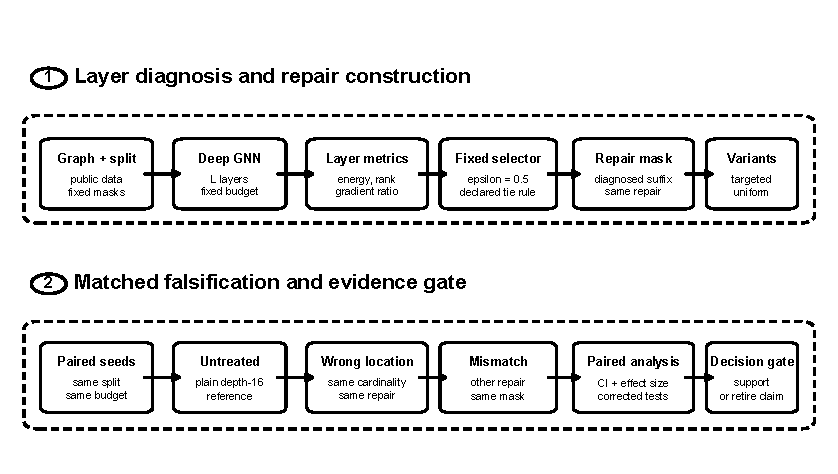
\includegraphics[width=0.97\textwidth]{figures/fig3_pipeline.pdf}
\caption{Operational pipeline used to construct and falsify the layer-repair rule. The first lane converts fixed graph data and layer diagnostics into matched intervention variants; the second lane compares paired seeds, wrong-location masks, and a mismatched repair before the evidence gate.}
\label{fig:pipeline}
\end{figure*}

\section{Real A6000 Pilot}

\subsection{Data and Fixed Protocol}

Cora was downloaded from the original Planetoid repository \cite{yang2016planetoid}. The public split contains 140 training nodes, 500 validation nodes, and 1,000 test nodes. Features were row-normalized. The graph was symmetrized, self-loops were added, and normalized sparse adjacency was used directly in PyTorch. No copied benchmark score was used.

Depths were 2, 4, 8, 16, and 32; hidden width was 64. Adam used learning rate 0.01 and weight decay $5\times10^{-4}$. Dropout was 0.5. Training ran for at most 300 epochs with validation patience 60, but epochs executed were not retained in the compact evidence. Seeds were 0, 1, and 2. The repair comparison fixed depth 16. Parameter count is $92{,}231+4{,}160L$, or 100,551 to 225,351 across the depth grid; repairs add no trainable parameters.

The same public test split was evaluated for all 27 conditions. Although validation selected checkpoints, the selector, threshold, and analysis were not locked before these test results were inspected. Test accuracy is therefore exploratory development evidence rather than an untouched estimate of final generalization. A confirmatory run must freeze code and analysis before one final test evaluation.

\subsection{Hardware and Provenance}

The evidence manifest records Linux 6.8.0-137-generic, Python 3.12.3, PyTorch 2.6.0+cu124, CUDA runtime 12.4, driver 595.84, and an NVIDIA RTX A6000 with compute capability 8.6. The process explicitly used \texttt{cuda:0}. PyTorch reported 50,896,240,640 device bytes. The full remote-manifest SHA-256 reported at execution was \texttt{edc663e03a4ef0f8\allowbreak 775e1ce64d16915b\allowbreak e4b7bd57ab86df96\allowbreak a7427e08031589d35}. The public repository contains the available compact 27-condition table and the exact 15-record depth-16 diagnostic subset.

\subsection{Depth Degradation}

\begin{figure}[t]
\centering
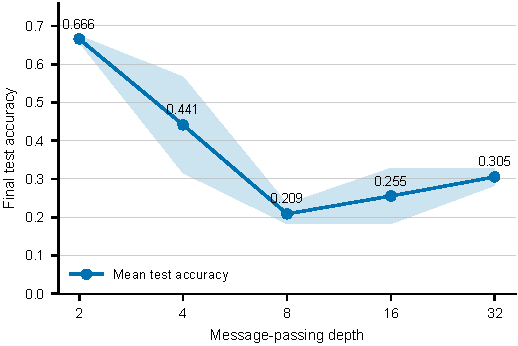
\includegraphics[width=\columnwidth]{figures/fig1_depth_accuracy.pdf}
\caption{Mean Cora test accuracy over three real training seeds. The shaded band is the sample standard deviation, not a confidence interval. Values are exploratory because the test set was repeatedly evaluated during development.}
\label{fig:depth}
\end{figure}

\begin{table}[t]
\caption{Plain-GCN Cora pilot over three seeds.}
\label{tab:depth}
\centering
\footnotesize
\begin{tabular}{rrrr}
\toprule
Depth & Mean accuracy & Sample SD & $n$ \\
\midrule
2 & 0.6660 & 0.0079 & 3 \\
4 & 0.4413 & 0.1250 & 3 \\
8 & 0.2087 & 0.0255 & 3 \\
16 & 0.2553 & 0.0725 & 3 \\
32 & 0.3053 & 0.0220 & 3 \\
\bottomrule
\end{tabular}
\end{table}

Table \ref{tab:depth} and Fig. \ref{fig:depth} show severe but nonmonotone degradation. Depth 2 is strongest, while all deeper untreated configurations are worse. The depth-16 to depth-32 increase does not rescue deep performance and illustrates why single-seed conclusions would be unreliable. These values are not competitive benchmark claims because the architecture and tuning budget were chosen to expose depth degradation.

\subsection{Repair Comparison and Failed Localization}

\begin{table}[t]
\caption{Depth-16 repair pilot with three paired seeds.}
\label{tab:repair}
\centering
\scriptsize
\setlength{\tabcolsep}{2pt}
\begin{tabular}{p{0.34\columnwidth}rrp{0.18\columnwidth}}
\toprule
Condition & Mean accuracy & Sample SD & Repair layers \\
\midrule
Plain & 0.2553 & 0.0725 & None \\
Targeted PairNorm & 0.5913 & 0.0595 & 2--16 \\
Uniform PairNorm & 0.5887 & 0.0592 & 1--16 \\
Wrong-location PairNorm & 0.6373 & 0.0580 & 15 layers \\
Mismatched residual & 0.5663 & 0.0607 & 2--16 \\
\bottomrule
\end{tabular}
\end{table}

The targeted-minus-wrong-location mean is $-0.0460$; its descriptive 95\% $t$ interval is $[-0.2979,0.2059]$, and paired Cohen's $d_z$ is $-0.4537$. Wrong-minus-targeted differences are $+0.163$, $-0.016$, and $-0.009$, so the mean reversal is dominated by seed 0. Exact sign-flip tests have only eight assignments at $n=3$ and are not confirmatory.

Targeted minus uniform is $0.0027$, with descriptive interval $[-0.0467,0.0520]$ and paired $d_z=0.1343$. Targeted minus the untuned residual mismatch is $0.0250$, with interval $[-0.2379,0.2879]$ and $d_z=0.2362$. Because tuning budgets were unequal, the latter comparison is not a fair prescription test. The pilot therefore supplies no evidence that targeting is better than treating every layer or that the selected repair type is superior.

Every repaired run exceeds its paired untreated depth-16 run, which is compatible with repair viability in this deliberately failing model. It does not establish that these measurements, this threshold, or this mapping identify where or how repair must be applied.

\subsection{Diagnostic and Execution Behavior}

At depth 16, effective rank crossed the 0.5 threshold at layer 2 for all three untreated seeds, and local gradient transmission also crossed at layer 2. Normalized energy crossed only near layers 15 or 16 for seeds 0 and 2 and did not cross for seed 1. The selector consequently chose PairNorm from layer 2 onward in every seed. The observables did not yield cleanly separated onset depths, and the diagnosed suffix treats 15 of 16 layers, leaving little opportunity for a meaningful efficiency advantage.

Peak PyTorch CUDA allocated memory was 73.8499 MB for plain, 104.8095 MB for targeted and wrong-location PairNorm, 106.8902 MB for uniform PairNorm, and 83.9967 MB for the residual mismatch. These are decimal megabytes of PyTorch allocated memory, not total or reserved board memory. Recorded elapsed time is not epoch time or matched throughput: the harness did not retain epochs executed, lacks a synchronized timing protocol, and includes validation, test evaluation, and the final diagnostic.

\begin{figure*}[t]
\centering
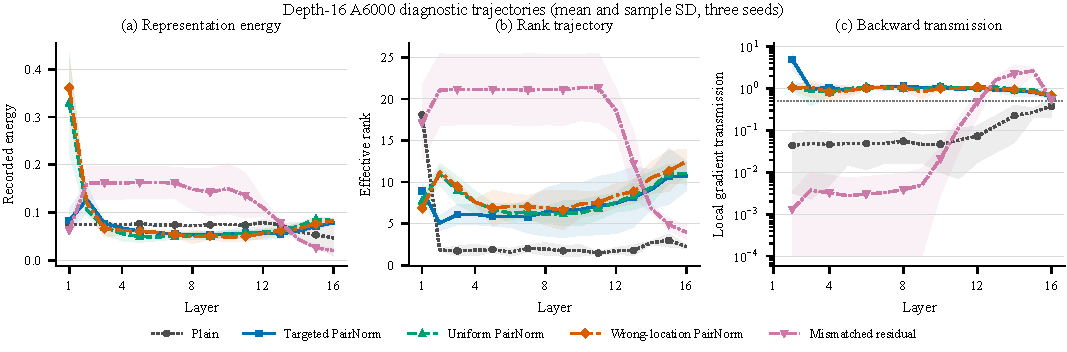
\includegraphics[width=0.98\textwidth]{figures/fig4_diagnostics.pdf}
\caption{Recorded depth-16 layer trajectories from the RTX A6000 evidence. Lines are seed means and shaded bands are sample standard deviations over three seeds, with no smoothing or interpolation. The dotted line in the gradient panel marks $\epsilon=0.5$.}
\label{fig:diagnostics}
\end{figure*}

\begin{figure*}[t]
\centering
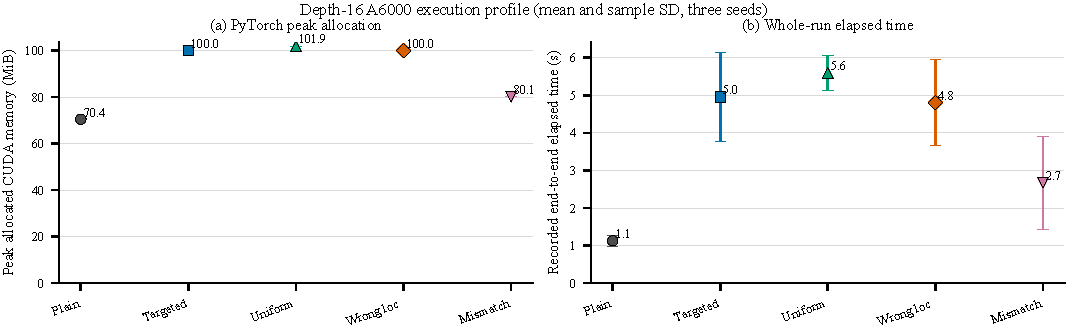
\includegraphics[width=0.98\textwidth]{figures/fig5_execution.pdf}
\caption{Recorded depth-16 PyTorch peak allocated CUDA memory and whole-run elapsed time from the same three RTX A6000 seeds. Elapsed time is neither per-epoch time nor synchronized throughput.}
\label{fig:execution}
\end{figure*}

\section{What the Pilot Falsifies}

The literature does not support the claim that smoothing, representation collapse, and gradient failure have never been considered jointly \cite{park2025fallacy,zhang2026rank,arroyo2025bridging}. Calling them independent channels would overstate novelty and causal identification.

A single forward threshold is directionally wrong for gradient norms. The local transmission statistic in \eqref{eq:gradient} is necessary, but the pilot shows that it may tie rank at an early layer. A confirmatory study should report continuous curves and threshold-free predictive measures in addition to $d^\star$.

The matched-cardinality wrong-location comparison is the primary falsification test. Because targeted repair does not outperform this weakly separated control, the present data do not establish that the diagnosed onset is causally privileged. Confirmatory masks must have substantially lower overlap while holding treatment cardinality and repair fixed.

\section{Confirmatory Protocol}

\subsection{Hypotheses and Data Regimes}

The confirmatory study follows a hierarchy. $H_1$ requires targeted repair to exceed untreated. $H_2$, the primary localization claim, requires targeted repair to exceed a family of low-overlap, same-cardinality masks using the same repair. $H_3$ requires the selected repair to exceed fairly tuned alternatives on the same mask. $H_2$ is tested only if $H_1$ passes, and $H_3$ only if $H_2$ passes. Datasets, masks, tuning budgets, seeds, contrasts, exclusions, stopping rules, and analysis code must be timestamped before final runs.

Homophilous node classification should use ogbn-arxiv as the principal dataset, with Coauthor CS/Physics and Amazon Computers/Photo as supporting datasets. Cora, CiteSeer, and PubMed remain sanity checks. Heterophily should use roman-empire, amazon-ratings, minesweeper, tolokers, and questions \cite{platonov2023heterophily}. Original Chameleon and Squirrel should be excluded. Graph-level long-range evaluation should use Peptides-func and Peptides-struct \cite{dwivedi2022lrgb}, with all baselines retuned under equal budgets \cite{tonshoff2023gap}. An ogbn-products neighbor-sampling run should test scale \cite{hu2020ogb}.

\subsection{Models, Tuning, and Statistics}

The minimum backbone set is plain GCN, GraphSAGE, GATv2, and GCNII. Depths are 2, 4, 8, 16, 32, and 64. Development uses three seeds only for code checks. Final seed count is determined by simulation or power analysis, with ten paired seeds as a minimum design target. Every method receives the same number of hyperparameter trials, validation metric, scheduler family, and early-stopping rule. Seeds, splits, and trial budgets are paired. Analysis uses seed-level differences, paired permutation tests, Holm correction over the declared contrast family, 95\% confidence intervals, and paired standardized effects. Development may inspect training and validation data only; the frozen model family is evaluated once on the held-out test split.

\subsection{Selector Robustness and Control Separation}

The full study sweeps $\epsilon\in\{0.3,0.4,0.5,0.6,0.7\}$ while retaining 0.5 as primary. It reports stability of $d^\star$ across seeds and early epochs. Threshold-free change-point and continuous-response models are secondary.

A localization test is identifiable only when controls differ materially from the target. The selector therefore uses a prespecified sparse budget of at most $L/2$ treated layers or a fixed-width contiguous window. Each wrong-location mask matches cardinality and repair type but must have Jaccard overlap at most 0.5 with the target; at least four such masks are sampled before outcomes are inspected. If no valid control family exists, the run may test repair viability but cannot contribute to a localization claim.

\subsection{Logging and Decision Gates}

Every epoch must write an append-only record containing dataset, backbone, depth, condition, seed, epoch, training loss, validation loss, training accuracy, validation accuracy, optimizer learning rate, epoch wall time, CUDA allocated bytes, and CUDA reserved bytes. The final record adds selected epoch, validation metric, one-time test metric, parameter count, FLOPs or measured operator count, and synchronized inference throughput. The release must include the complete manifest, raw records, commands, configuration, environment lockfile, dataset hashes, checkpoint hashes, predictions, and plotting code.

\begin{table}[t]
\caption{Decision gates for confirmatory runs.}
\label{tab:gates}
\centering
\scriptsize
\setlength{\tabcolsep}{2pt}
\begin{tabular}{p{0.20\columnwidth}p{0.43\columnwidth}p{0.25\columnwidth}}
\toprule
Gate & Pass criterion & If failed \\
\midrule
Reproduction & Published-range shallow baseline & Stop pipeline \\
Control separation & Equal cardinality; Jaccard at most 0.5 & No location test \\
Location & Targeted exceeds low-overlap controls & Retire localization \\
Matching & Selected repair exceeds tuned alternatives & Retire prescription \\
Efficiency & Noninferior accuracy and lower cost & Drop efficiency claim \\
\bottomrule
\end{tabular}
\end{table}

\section{Reproducibility and Code Availability}

The public artifact repository\footnote{\href{https://github.com/kacytran1122/falsification-guided-layer-repair}{Falsification-Guided Layer Repair GitHub repository}} contains the training harness, the compact 27-condition evidence table, the exact 15-record depth-16 diagnostic subset, plotting programs, figures, the LaTeX manuscript, and environment requirements. The local diagnostic subset has SHA-256 \texttt{c1905c5feb70d6865\allowbreak e2e1b3f1bce31080\allowbreak c85ccebc1c2ef57a\allowbreak 45c4668bc658c61}. The available bundle does not contain raw epoch records, the complete 27-record per-layer manifest, standard output and error logs, checkpoints, or an environment lockfile from the executed remote environment. Reproducibility is therefore limited to the released evidence and figure regeneration, not full retraining equivalence.

The repository uses interpretable names and records exact dataset, method, hardware, and analysis provenance. Authorship, institutional clearance, conflicts of interest, dataset licenses, and disclosure of any AI assistance remain author responsibilities.

\section{Limitations}

This pilot has one small homophilous dataset, one plain backbone, three seeds, and no tuning. Its depth-2 result is below commonly reported tuned GCN performance, so it is not a benchmark reproduction. The wrong masks overlap 14 of 15 targeted layers. No per-epoch loss, accuracy, memory, learning-rate, or timing history was retained, so learning curves and convergence comparisons cannot be reconstructed. The same test split was evaluated for all conditions before the study was locked, making all reported test values exploratory.

The pilot does not measure oversquashing directly. Structural curvature or long-range sensitivity should be treated as explanatory covariates rather than replaced by energy, rank, or gradient statistics. Node-specific adaptive depth is deferred because existing methods already address it and because the global localization premise has not passed its own control.

\section{Conclusion}

The released evidence records real RTX A6000 training and a negative localization result. Deep plain GCNs degraded on Cora, and repairs were viable in this deliberately failing model, but targeted repair was indistinguishable from uniform repair and did not outperform the weakly separated wrong-location control. The selected repair was not fairly tested against alternatives, efficiency was not measured at epoch level, and the test set was not untouched. The defensible contribution is a corrected diagnostic definition, a claim hierarchy, and a falsification protocol that exposes what the pilot cannot establish. Publication as an effectiveness paper requires the confirmatory study; otherwise the work remains a negative pilot and protocol.

\bibliographystyle{IEEEtran}
\bibliography{references}

\end{document}
